% Author: Dominic van der Zypen
\documentclass[12pt, a4paper]{amsart}
\usepackage{tikz}
\usetikzlibrary{topaths,calc}

\addtolength{\hoffset}{-1cm} % --> Umstellung A4
\addtolength{\textwidth}{2cm}
\addtolength{\voffset}{-1cm}
\addtolength{\textheight}{2cm}

%\textheight=645pt
\usepackage{amssymb}
\usepackage{amsthm}
\usepackage{amsfonts}

\newtheorem{lemma}{Lemma}[section]
\newtheorem{theorem}[lemma]{Satz}
\newtheorem{corollary}[lemma]{Korollar}

\theoremstyle{definition}
\newtheorem{definition}[lemma]{Definition}
\newtheorem{remark}[lemma]{Bemerkung}
\newtheorem{example}[lemma]{Beispiel}
\newtheorem{conjecture}[lemma]{Vermutung}
\newtheorem{exercise}[lemma]{\"Ubung}
\newcommand{\C}{\text{Config}}

%-----------------------------------
\begin{document}
\parskip = 2mm
\parindent = 0mm

\begin{center}
    \textbf{\Large ${\bf P}$ vs ${\bf NP}$ \\ for the (formalist-leaning) mathematician}
\end{center}

\vspace*{3mm}

\begin{center}
Dominic van der Zypen
\end{center}

\section{Introduction}
I have long had an iffy feeling about the formulation of the ${\bf P}$ vs {\bf NP} problem. 
I sort-of know Turing machines, I have a vague concept of what is "a class of problems", 
and I have heard many times that {\bf NP} is the class of problems for which a solution 
can be checked in polynomial time for correctness.

All my ifs-and-buts add to a quite shaky view - and I decided to get to the bottom of 
things and provide a rigorous and (hopefully) mathematically appealing definition of 
Turing machines, languages, and the like. 

%-------------
\section{Configurations}

Let $ \omega$ denote the first infinite ordinal (which can be thought 
of as $ \mathbb{N}$, the set of non-negative integers). Recall that each
$n \in \omega$ is an {\em ordinal}, that is, $0:=\emptyset$ and for $n>0$,
its members are the numbers $ 0,\ldots, n-1$, so $ n = \{0,\ldots,n-1\}$. 
We write $n^\omega$ for the collection of all maps $f:\omega \to n$. 

Our first 
central concept, the {\bf configuration}, is the mathematical model of the 
notion of the {\bf tape} of the Turing machine, together with the {\bf writing 
head} and the {\bf internal state} of the machine. 

We fix a finite set $Q$ such that $Q \cap \omega = 0$ and refer to $Q$ as the
{\em set of states}. $Q$ has two special states, called {\em accept} and 
{\em reject}. 

\begin{definition} A {\em configuration} is a triple $C = (q, h, t) \in
    Q \times \omega \times 3^\omega$  (where $3 = \{0,1,2\}$) such that the
    sequence (function) $t:\omega\to 3$ is eventually constant with value $2$. (This means
    that there is $N\in \omega$ such that $c(k) = 2$ for all $k\in \omega$ 
    with $k\geq N$.) The collection of configurations over the set of states $Q$ 
    is denoted by $\C(Q)$.
\end{definition}

{\bf Remarks.} The letter $t$ stands for "tape". 
We interpret $2$ as being the {\em blank} symbol. The {\em value} symbols
are 0 and 1. The blank symbol 2 can be used to separate "input strings" consisting of 0,1.
The value $h\in \omega$ can be thought of as the position of the {\em head} of the 
Turing machine, and $q\in Q$ is the current state.

%--- bildli ---
\begin{center}
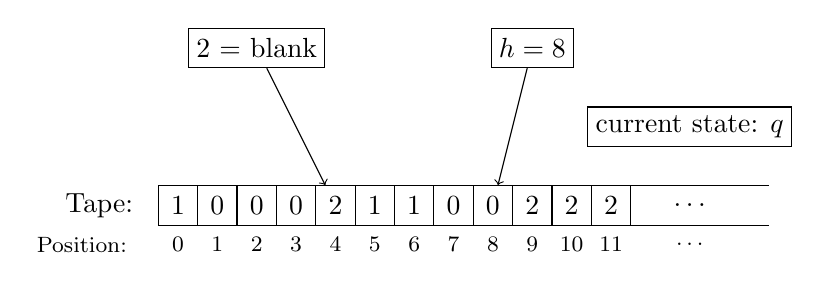
\begin{tikzpicture}[
   box/.style={rectangle,draw,minimum width=0.5cm,
    minimum height=0.5cm,inner sep=+0.1cm}
    ]

    % Boxes:
    \node at (0,1) {Tape:};
    \node[box] at (1,1) (h0) {1};
    \node[box] at (1.5,1) (h1) {0};
    \node[box] at (2,1) (h2) {0};
    \node[box] at (2.5,1) (h3) {0};
    \node[box] at (3,1) (h4) {2};
    \node[box] at (3.5,1) (h5) {1};
    \node[box] at (4,1) (h6) {1};
    \node[box] at (4.5,1) (h7) {0};
    \node[box] at (5,1) (h8) {0};
    \node[box] at (5.5,1) (h9) {2};
    \node[box] at (6,1) (h10) {2};
    \node[box] at (6.5,1) (h11) {2};
    \node at (7.5, 1) (h16) {$\ldots$};

    % Positions:
    \node at (-0.22,0.5) {\footnotesize{Position:}};
    \node at (1,0.5) {\footnotesize{0}};
    \node at (1.5,0.5) {\footnotesize{1}};
    \node at (2,0.5) {\footnotesize{2}};
    \node at (2.5,0.5) {\footnotesize{3}};
    \node at (3,0.5) {\footnotesize{4}};
    \node at (3.5,0.5) {\footnotesize{5}};
    \node at (4,0.5) {\footnotesize{6}};
    \node at (4.5,0.5) {\footnotesize{7}};
    \node at (5,0.5) {\footnotesize{8}};
    \node at (5.5,0.5) {\footnotesize{9}};
    \node at (6,0.5) {\footnotesize{10}};
    \node at (6.5,0.5) {\footnotesize{11}};
    \node at (7.5, 0.5) {\footnotesize{$\ldots$}};

    % ... etc-lines:

    \draw (6.5,1.25) -- (8.5,1.25);
    \draw (6.5,0.75) -- (8.5,0.75);

    % blank / head / state

    \node[box] at (2, 3) (b){$2$ = blank};
    \node[box] at (5.5, 3) (head) {$h = 8$};
    \node[box] at (7.5, 2) (state) {current state: $q$};

    % arrows

    \draw[->] (b) -- (h4);
    \draw[->] (head) -- (h8);

\end{tikzpicture}
\end{center}
%--- bildli ---

%--------------
\section{Turing machines}
We are ready for the central notion -- maybe of computer science:

\begin{definition}
A {\em Turing machine} is a tuple $(Q, \delta)$, such that 
\begin{itemize}
\item $Q$ is a finite set 
    with $Q\cap \omega = \emptyset$ containing two special elements
{\em accept} and {\em reject}, and
\item $\delta: Q\times \{0,1,2\} \to Q \times \{0,1,2\} \times \{-1,1\}$ is a function 
    with the following property: if $q \in \{${\em reject, accept}$\}$ 
        and $b\in \{0,1,2\}$, then $\delta(q,b) = (q,b,-1)$.
        If $\delta(q,b) = (q', b', s)$ for $q,q'\in Q, b,b'\in \{0,1,2\}$ and 
        $ s\in \{-1,1\}$
        we write
        \begin{itemize}
            \item $\text{state}(\delta(q,b)) = q'$,
            \item $\text{output}(\delta(q,b)) = b'$, and
            \item $\text{step}(\delta(q,b)) = s\in\{-1,1\}$. 
        \end{itemize}
\end{itemize}
    The function $\delta$ is called the {\em transition function} and can 
    be looked at as the "clockwork" of the Turing machine.
\end{definition}

Time for the synthesis: combining configurations and Turing machines!

We need the following {\em convention}: if $n\in\omega$, define the function 
$\text{pred}:\omega\to \omega$ by $0 \mapsto 0$ and $n \mapsto n-1$ for $n\in\omega
\setminus\{0\}$. By slight abuse of notation, we write $n-1$ instead of 
$\text{pred}(n)$ for all $n\in \omega$.

\begin{definition}
    Let $T=(Q,\delta)$ be a Turing machine, $T$ induces a {\em configuration
    map} $${\frak C}_T: \C(Q)\to \C(Q)$$ in the following way:

    If $C = (q,h,c)\in \C(Q)$ then ${\frak C}_T\big((q,h,c)\big) = (q', h', c')$
    where
    \begin{itemize}
        \item $q' = \text{state}\big(\delta(q, c(h))\big), $\footnote{recall
            that $c(h)$ is the value of the configuration at head position $h$.}
        \item $h' = h + \text{step}\big(\delta(q, c(h))\big)$, and 
            \footnote{remember that $\text{step}\big(\delta(q,c(h))\big)\in\{0,1\}$, and $0 - 1 = 0$ in
            our convention.}
        \item $c': \omega \to \{0,1,2\}$ is defined by $c'(h) = \text{output}\big(\delta(q, c(h))\big)$
            and $c'(x) = c(x)$ for all $x\in \omega\setminus \{h\}$. 
            \footnote{that is $c'$ agrees 
            with $c$ except possibly on the head position $h$.}
    \end{itemize}

\end{definition}
\end{document}
